% This is a template for your written document.
%
% To compile using latexmk on the command line, run the following: 
% latexmk -pdf main.tex

\documentclass[12pt]{article}
\usepackage{setspace}
\singlespace
\usepackage[left=1in,right=1in,top=1in,bottom=1in]{geometry}

\title{\textbf{MCP for Handwriting Recognition}}
\author{Miles Fike}
\usepackage{graphicx}
\graphicspath{{./images/}}

\begin{document}

\maketitle

In the past, many different computer visions systems have been created to convert handwritten or printed text of different fonts and styles to computer readable text. These systems all tend to involve similar principles of computer vision to decipher text using systems trained on data sets of images of text. More recently Model Context Protocol (MCP) has been released. As is explained on the Model Context Protocol Website, this technology assists AI systems use of technologies by providing connections between AI systems and tools, workflows, and data sources that they need \cite{modelContextProtocol/getting-started/intro}. I intend to approach issues and limitations of transcription technologies through the implementation of MCP, so that more specific AI models can be chosen to convert different fonts and handwriting systems to digital text rather than having one large very general system for all types of text. 

Currently many different computer vision systems are used to interpret handwriting as digital text, but these systems are somewhat constrained.  For example, two researchers, Ying Yu and Yuhe Tian, at College of Design and Art Shenyang Architecture University created a computer vision system that interpreted handwritten numbers based on a data set of handwritten numbers. They noticed that when faced with “more than one handwritten digits written in succession and handwritten digits with incoherent strokes” the tool was less accurate \cite{10.1145/3727648.3727679}. The limitations of the training led to the AI failing to recognize some characters. To get around issues like these, I could attempt to have a computer vision system based on a data set of densely packed characters accessible to the MCP. Using this data would help the system focus on interpreting dense characters. Another computer vision system created by Bensalah et al. and for their article, “A User Perspective on HTR Methods for the Automatic Transcription of Rare Scripts: The Case of Codex Runicus” focused on obscure scripts, using alternative methods as “existing methods are often too constrained since they need labelled data for training and fine-tuning.” \cite{10.1145/3519306}  To get around this issue, they focused on alternative few-shot method to detect characters without a dataset. This technique could help me to analyze more obscure handwriting styles with computer vision while more advanced computer vision systems may be implemented for more popular writing styles. It is important to note that many datasets and handwriting recognition systems exist across the internet, so I should be able to create diverse systems to handle most tasks. My system will involve aspects of several different systems using the Model Context Protocol to decide between them for specific cases.

The vast majority of my computer vision systems will be implemented using convolution frames. As is described by Soonhoi Ha and Eunjin Jeong, in their article “Software Optimization and Design Methodology for Low Power Computer Vision Systems” Within these frames a convolution kernel “slides along the input matrix for the layer, the convolution operation generates a feature map” which is used as the input to the next layer and eventually compared with the learned knowledge of the system \cite{10.1145/3687310}. The primary difference between these systems will be the implementation of different data sets in the learning processes of each different computer vision system. There is no reason that the same basic system could not be used for all well-known writing systems for which I have access to thorough annotated data sets.

For the implementation of this project, I will create a simple web app allowing for image and optional text input. The image input will take the image of the text while the optional text box would allow for a description of the writing style, skipping the optional computer vision to detect a specific writing style. From here, the file will be run through the required computer vision system or systems to convert it to plain text by MCP an MCP Client sending the image to the MCP server for the determined writing style. This will be returned to the user in the form of a text file that they can download.
    \begin{figure}[htbp]
        \centering
		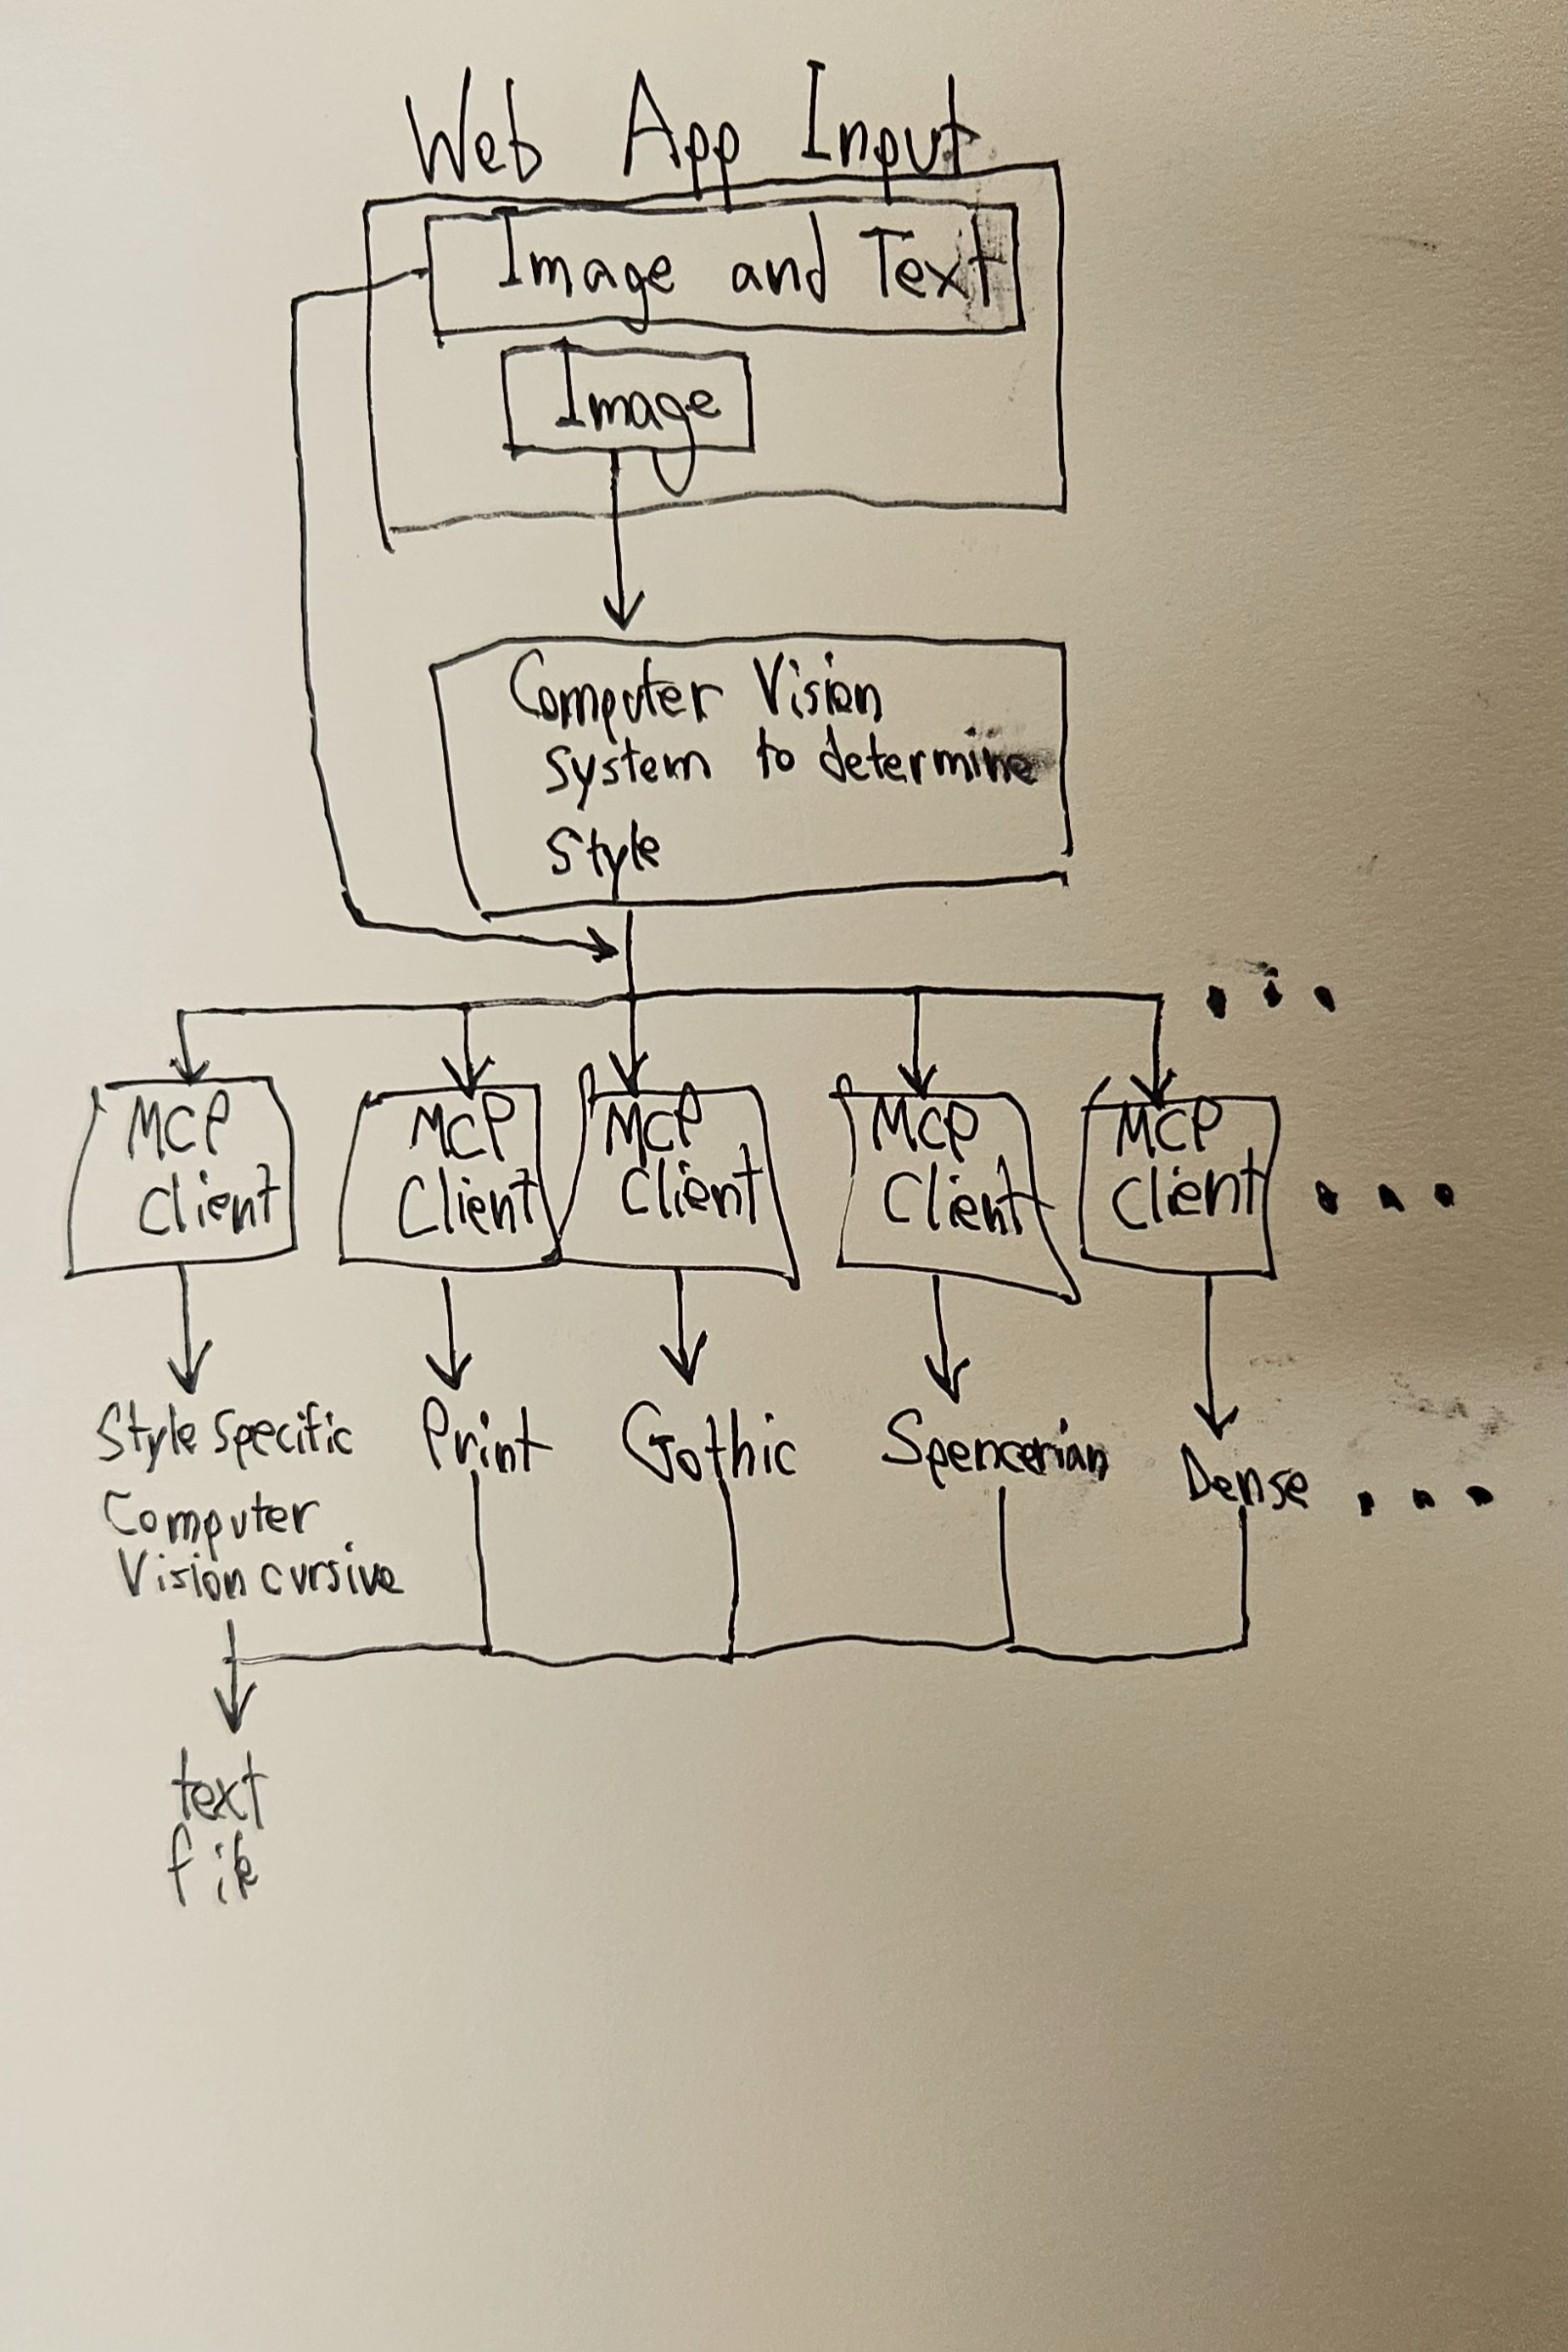
\includegraphics[width=0.8\textwidth]{./1000026679.jpg}
        \caption{Depiction of the planned app functionality.}
        \label{fig:myfigure1}
    \end{figure}
	\begin{figure}[htbp]
        \centering
		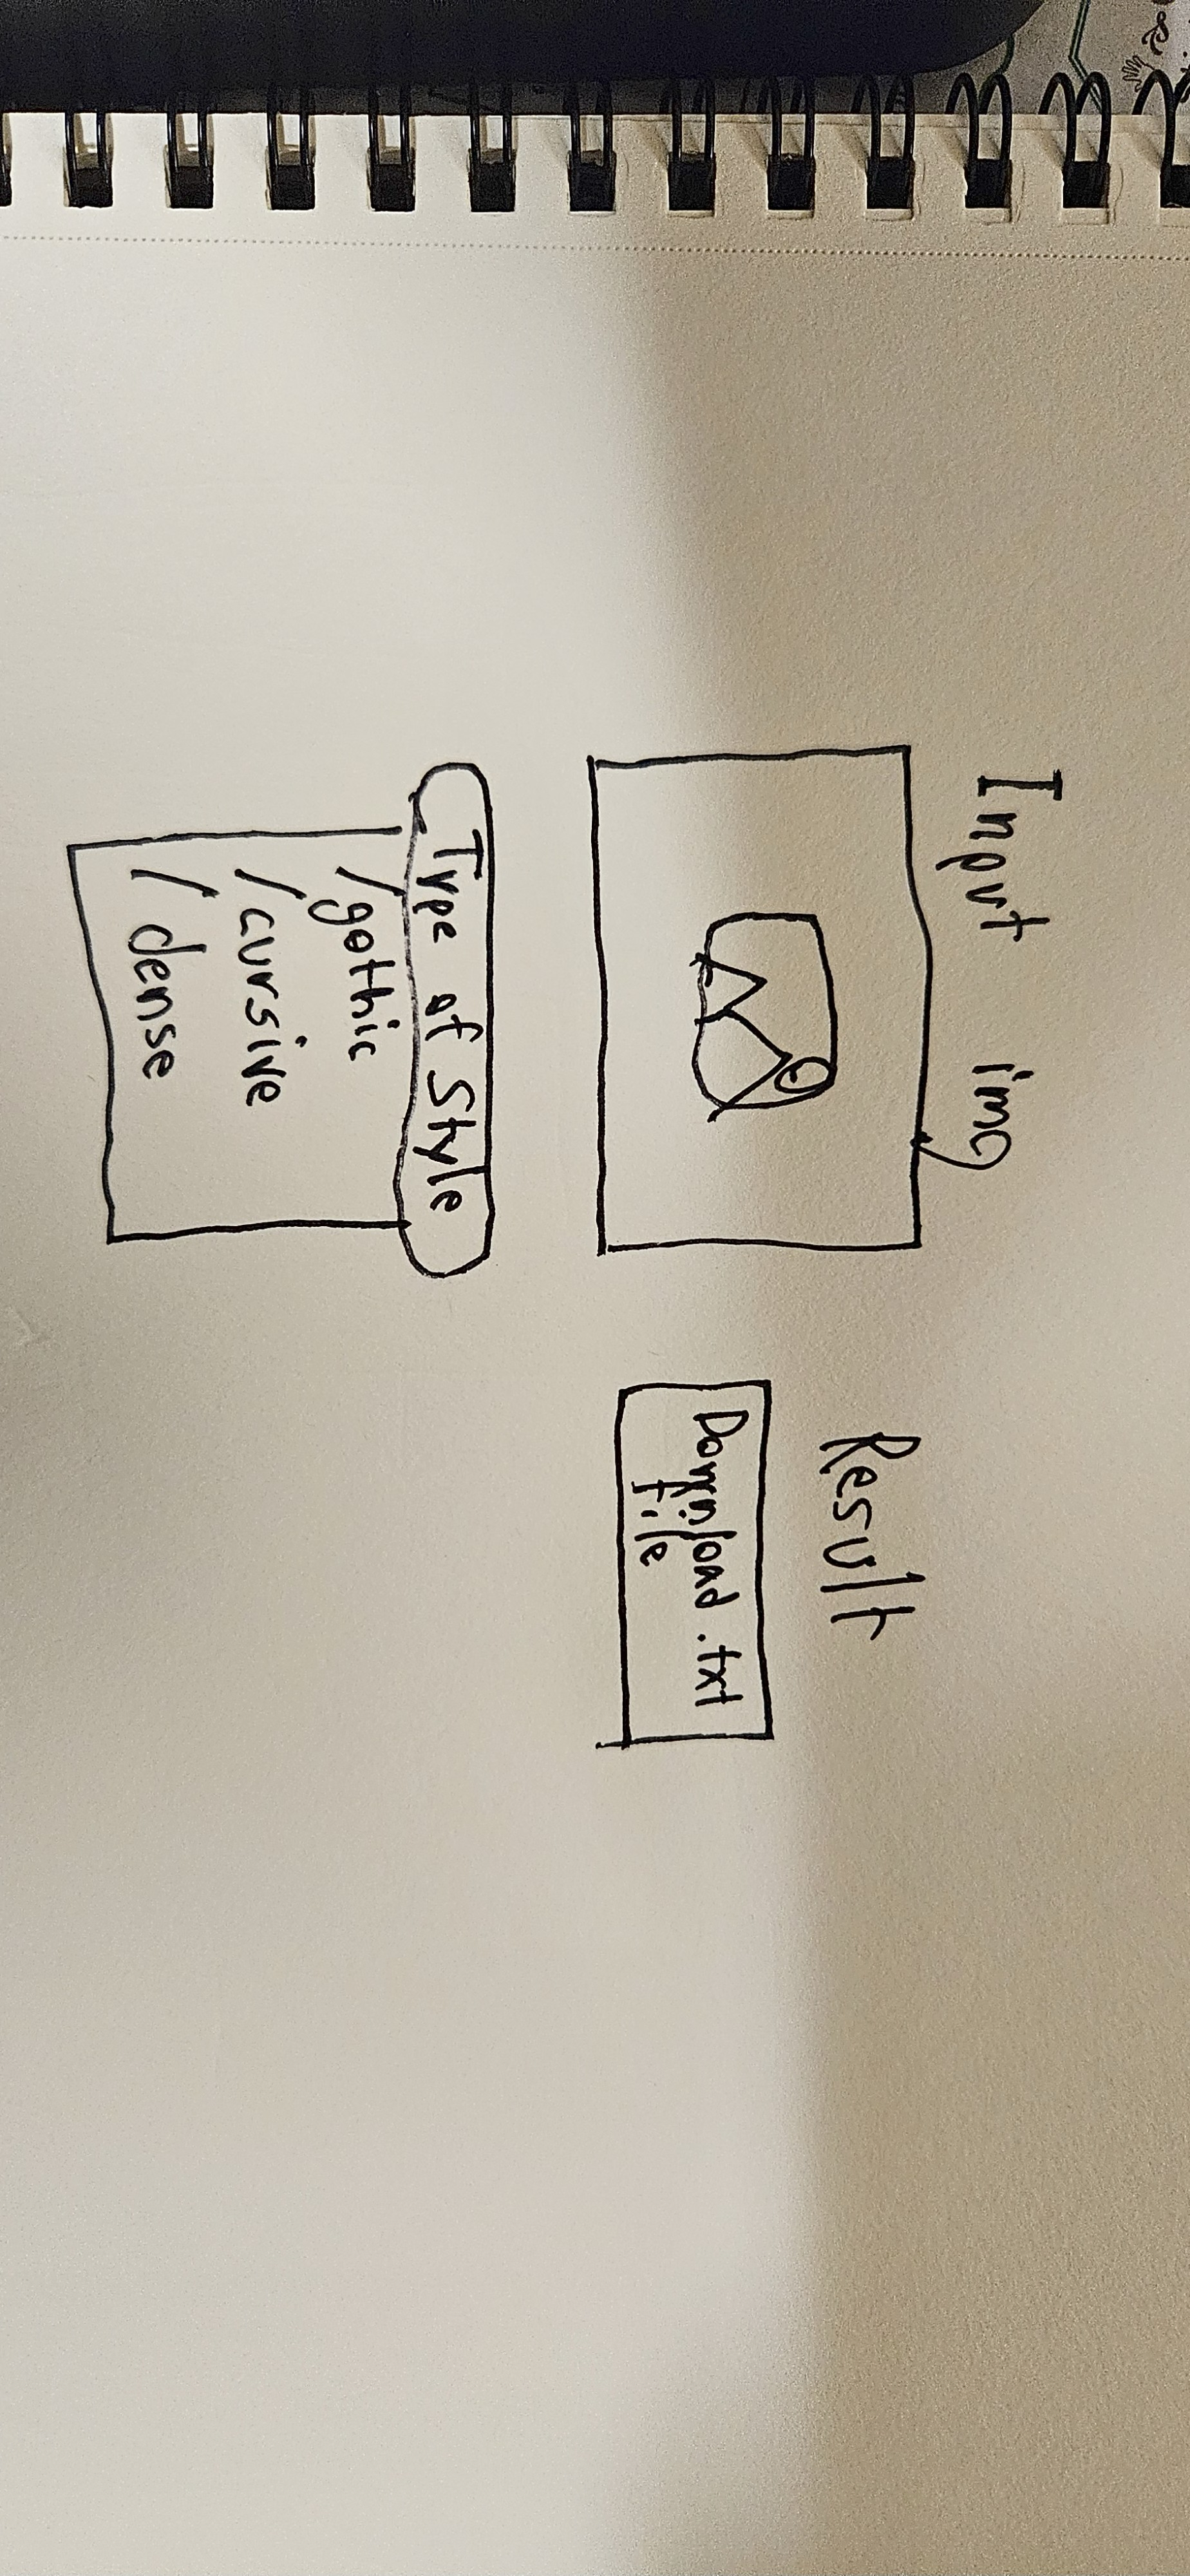
\includegraphics[width=0.8\textwidth]{./jp.jpeg}
        \caption{Depiction of the planned user interface.}
        \label{fig:myfigure1}
    \end{figure}
\newpage
\section*{Appendix}
\begin{itemize}
	\item Computer vision systems return digital text from images of handwritten text, at least 3.
	\item User can view the extracted text.
	\item A text input allows the user to select the style of the text.
	\item MCP determines the best model for text extraction based on the image provided.
	\item User can select a specific model for text extraction.
	\item System provides feedback on the accuracy of the text extraction.
	\item Drop box to upload an image for text extraction.
	\item A button downloads the text into a text file.
	\item A text box displays the tool used to read the text to clarify to the user what model was used.
\end{itemize}


\bibliographystyle{acm}
\bibliography{bibliography.bib}

\end{document}
